\documentclass[border = 5mm]{standalone}
%\documentclass[dvisvgm]{minimal}

\usepackage{tkz-euclide}

\usepackage[OT1]{fontenc}
\usepackage{sansmathfonts}


\begin{document}
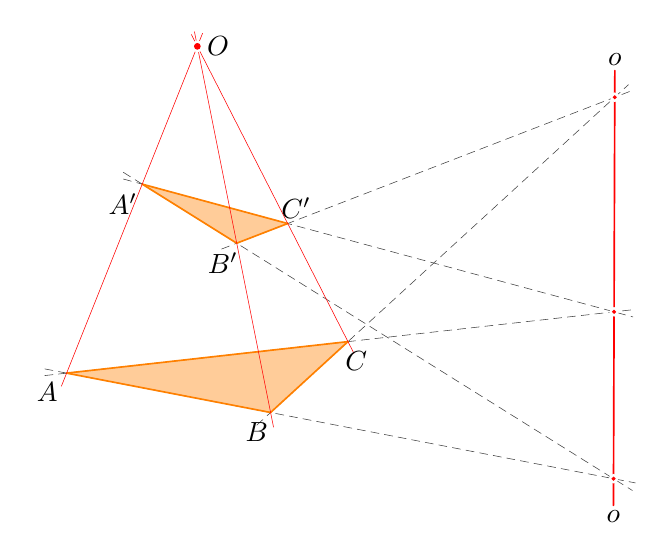
\begin{tikzpicture}
	
% Point O, triangles ABC and A'B'C'
\tkzDefPoints{2/5/O, 0/0/X, 3/0/Y, 4.55/0/Z}

\tkzDefPointOnLine[pos=0.35](O,X) \tkzGetPoint{A'}
\tkzDefPointOnLine[pos=0.5](O,Y) \tkzGetPoint{B'}
\tkzDefPointOnLine[pos=0.45](O,Z) \tkzGetPoint{C'}

\tkzDefPointOnLine[pos=0.83](O,X) \tkzGetPoint{A}
\tkzDefPointOnLine[pos=0.93](O,Y) \tkzGetPoint{B}
\tkzDefPointOnLine[pos=0.75](O,Z) \tkzGetPoint{C}

\tkzFillPolygon[orange, opacity=0.4](A,B,C)
\tkzFillPolygon[orange, opacity=0.4](A',B',C')


% Points common to corresponding sides of the triangles
\tkzInterLL(A,B)(A',B') \tkzGetPoint{L}
\tkzInterLL(A,C)(A',C') \tkzGetPoint{M}
\tkzInterLL(B,C)(B',C') \tkzGetPoint{N}

\tkzDrawLines[gray!150, add = 0.04 and 0.04, densely dashed, very thin](A,L A',L A,M A',M B,N B',N)

% Line through the three points
\tkzDrawLines[red, add = 0.07 and 0.07, semithick](L,N)

% Highlight the sides of the triangles
\tkzDrawSegments[semithick, orange](A,B A,C B,C)
\tkzDrawSegments[semithick, orange](A',B' A',C' B',C')

% Draw projection lines
\tkzDrawLines[red, add = 0.04 and 0.04, very thin](O,A O,B O,C)

% Label points and line
\tkzDrawPoints[color=white, size=3](L,M,N)
\tkzDrawPoints[color=red, size=1](L,M,N) 
\tkzDrawPoints[color=white, size=4](O)
\tkzDrawPoints[color=red, size=2](O)

\tkzLabelPoints[right](O){O} 
\tkzLabelPoints[xshift=-7pt](A,A')
\tkzLabelPoints[xshift=-5pt](B,B')
\tkzLabelPoints[xshift=3pt](C)
\tkzLabelPoints[xshift=3pt, yshift=13pt](C')

\tkzLabelLine[pos=-0.1](L,N){$o$}     
\tkzLabelLine[pos=1.1](L,N){$o$}


		
\end{tikzpicture}
\end{document}